\chapter{Slot Menu:}

The Slot Menu is an important sub-menu of the Grid Page and is used to manipulate slots in a variety of ways.\\\\
It can be used to clear one or more slots in a row, to merge  MD sequencer data in to the internal sequencer or to configure a slot's chain settings. It also provides a quick way to activate or deactivate various Global Chain Modes.
\\\\
%\begin{center}
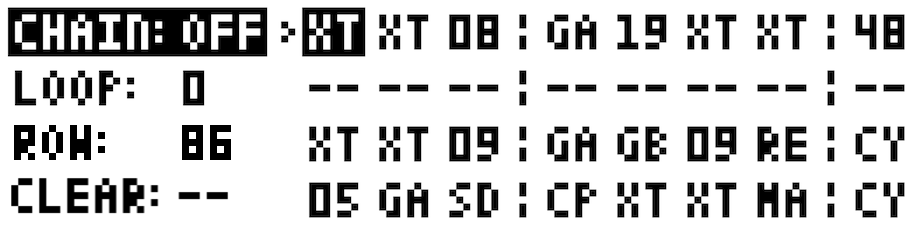
\includegraphics[scale=.35]{slot_menu.png}
%\end{center}
\\\\
\textit{The SlotMenu is accessible from the GridPage by holding down the  \textbf{[Shift2]} function 
button. When  \textbf{[Shift2]}  is released, any changes to the menu will be applied to the current slot. If the APPLY value is greater than 1, changes will be applied sequentially; starting from the current slot and up to the number of slots specified by the APPLY value}
\\\\
\textit{For users running MCL on a \textbf{HD44780 LCD}, the SlorMenu  is accessible from the GridPage by holding down the  \textbf{[Shift2]} function button and pressing a corresponding encoder button. For example if slots 5 to 8 are displayed on screen, holding  \textbf{[Shift2]} and then pressing \textbf{[Encoder3]} will open the slot menu for slot 7.}

\section{Slot Menu Options:}
Slot Menu has following options and selectable values:
\begin{itemize}

\item{Chain: [ --, auto, manual, random ]}

\subitem{- auto: enables chain auto mode global setting}
\subitem{- manual: enables chain manual mode global setting}
\subitem{- random: enables chain random mode global setting}

\item{Loops:  (0, 64)}
\subitem{- specify how many times to loop track/slot}
\item{Row:    (0,127)}
\subitem{- specify which row, the current slot is to load/jump to after n loops.}
\item{Seq: [ --, merge ]}
\subitem{ -merge slot's MD sequencer data in to the internal sequencer}
\item{Clear: [ --, YES ]}
\subitem{- clear the selected slot.}
\item{Apply: (0,20)}
\subitem{- apply the above changes to the next N slots upon exit of SlotMenu.}

\end{itemize}

